\documentclass{article} %Classe del documento
\usepackage{float}  %Permette di posizionare le immagini dove si vuole
\usepackage{booktabs} %Permette di creare tabelle con linee orizzontali
\usepackage[svgnames]{xcolor} %Permette di usare i colori
\usepackage{listings} %Permette di inserire codice R nel documento
\usepackage{upquote} %Permette di usare i singoli apici
\usepackage{graphicx} %Permette di inserire immagini
\usepackage{verbatim} %Permette di inserire commenti multiriga
\usepackage[a4paper, left=1.60in, right=1.60in, top=1.7in, bottom=1.7in]{geometry}
%\usepackage[a4paper, margin=1.6in]{geometry}
\usepackage{changepage} %Permette di regolare i margini
\usepackage[utf8]{inputenc} %Permette l'uso dei caratteri accentati
\usepackage[italian]{babel} %Permette l'uso della la lingua italiana
\usepackage{setspace}
\usepackage{graphicx}
\usepackage{tabularx}
\usepackage{caption}
% \title{\texttt{Mussels}}
% \author{Stefano Terrone e Leonardo Perin}
% \date{20 gennaio 2025}

\begin{document}

%Aggiunge spaziatura di 1.5
\onehalfspacing

% \maketitle

\newpage
% \begin{flushleft}
%     %\vskip 50pt
% \textbf{\Large 0.1 \: Introduzione}    
% \end{flushleft}

% \vskip 10pt

% \hspace{0.20in}
% il database è composto da \textbf{n} variabili:
% \begin{itemize}
%     \item \texttt{}: 
%     \item \texttt{}: 
%     \item \texttt{}: 
%     \item \texttt{}:  
%     \item \texttt{}: 
%     \item \texttt{}:
%     \item \texttt{}:
% \end{itemize}
% Le analisi sono state eseguite con il software R nella versione 4.2.3.\\ Il livello di significatività è fissato al 5\%.
% \vskip 55pt 

\newpage
\begin{flushleft}
    %\vskip 30pt
    \textbf{\Huge 1. \: Analisi esplorative}
    \vskip 30pt
    %Prima parte: analisi univariate
    %Titolo
    \textbf{\Large 1.1 \: Analisi Univariate}
\end{flushleft}
\vskip 10pt

La Hydronium concentration è l'operazione inversa per trovare il pH, ed è la concentrazione di idronio


%Introduzioni analisi esplorative
Il database è composto da 44 osservazioni, una per ciascun fiume, e 9 varabili. Le varabili rappresentano varie caratteristiche dei fiumi come il numero di specie di cozze presenti, la dimensione del fiume, la distanza da alcuni fiumi importanti, e vari indicatori sulla qualità delle acque.\\

%Tabella di sintesi
\begin{table}[H]
    \centering
    \renewcommand{\arraystretch}{1.4} % Increases the row height
    \begin{tabularx}{\textwidth}{p{69pt}l p{30pt}c p{45pt}c p{35pt}c p{40pt}c p{30pt}c p{27pt}r}
        \toprule
        & Min. & 1\textsuperscript{0} qt. & Mediana(IQR) & Media(sd) & 3\textsuperscript{0} qt. & Max\\
            \midrule  
            \texttt{Species} & 2.00 & 8.00 & 10.00(5.0) & 11.25(5.99) & 13.00 & 33.00 \\
            \texttt{Area} & 349 & 2115 & 4315(7797.5) & 6590(6016) & 9912 & 27900 \\
            \texttt{Stepping}\\ \texttt{stones to AC} & 1.00 & 7.00 & 15.50(15.25) & 15.34(9.19) & 22.25 & 33.00 \\
            \texttt{Stepping }\\
            \texttt{stones to AP} & 0.00 & 4.00 & 12.00(14.25) & 12.02(8.24) & 18.25 & 28.00 \\
            \texttt{Stepping }\\
            \texttt{stones to SV} & 0.00 & 5.00 & 7.00(13.25) & 8.136(8.94) & 11.00 & 21.00 \\
            \texttt{Stepping }\\
            \texttt{stones to SL} & 4.00 & 16.75 & 22.00(0.775) & 22.16(1.84) & 30.00 & 36.00 \\
            \texttt{Nitrate} & 0.100 & 0.600 & 0.800(0.775) & 1.495(1.84) & 1.375 & 8.700 \\
            \texttt{Solid Residue} & 29.0 & 56.5 & 78.0(64.0) & 112.4(17.3) & 120.5 & 520.0 \\
            \texttt{Hydronium} & 0.200 & 1.00 & 1.600(2.2) & 3.631(6.03) & 3.200 & 32.00 \\
            \texttt{ln(Area)} & 5.855 & 7.657 & 8.370(1.54) & 8.331(1.07) & 9.201 & 10.24 \\
        \bottomrule
    \end{tabularx}
    \caption{Tabella di sintesi}
\end{table}
%Introduzione analisi univariate

%Esempio di analisi univariata su una variabile
%Titolo
% \newpage
% \begin{center}
% \textbf{\large }
% \end{center}

%Grafico delle variabili univariate
% \begin{figure}[H]
%     \centering
%     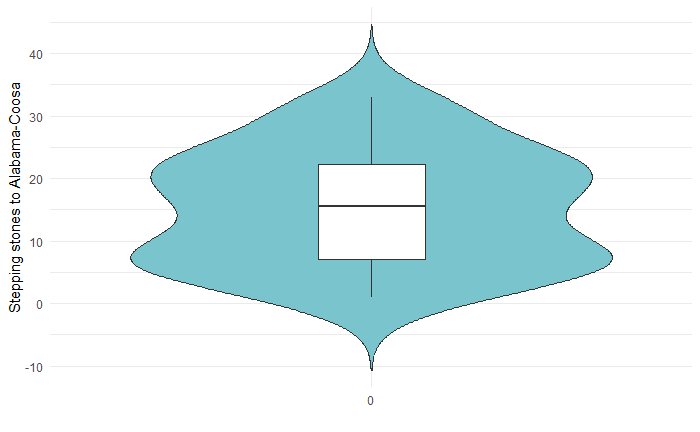
\includegraphics[width=0.6\textwidth]{immagini/vp_ac.png}
%     \caption{}
% \end{figure}

% \begin{figure}[H]
%     \centering
%     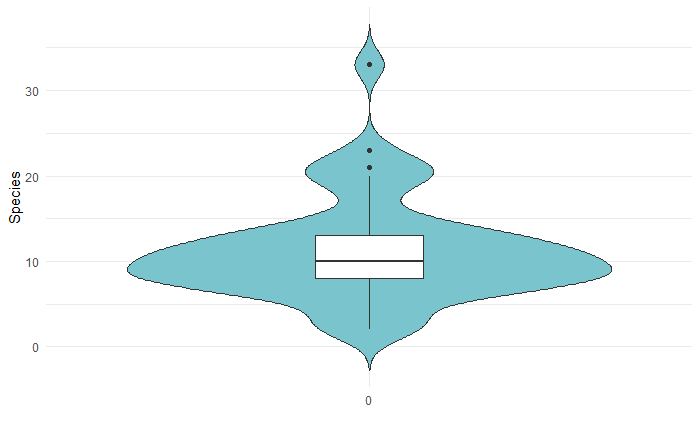
\includegraphics[width=0.47\textwidth]{immagini/vp_species.png}
%     \hspace{0.04\textwidth}% Distanza tra le immagini
%     \includegraphics[width=0.47\textwidth]{C:/Users/Stefa/Documents/1-Stefano/1-Medica/Lab10/grafici/4.png}
%     \caption{A sinistra: curve di sopravvivenza di Kaplan-Meier.\\ A destra: curve di sopravvivenza basato sulla trasformazione complementare del logaritmo log-log.}
% \end{figure}

\begin{figure}[H]
    \centering
    \begin{minipage}{0.49\textwidth}
        \centering
        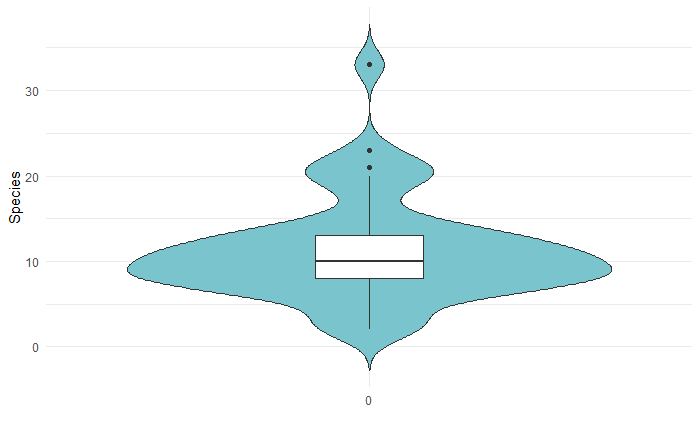
\includegraphics[width=\textwidth]{immagini/vp_species.png}
        \captionsetup{justification=centering}
        \caption{Violinplot della variabile \texttt{Species}}
    \end{minipage}
    \hfill
    \begin{minipage}{0.49\textwidth}
        \centering
        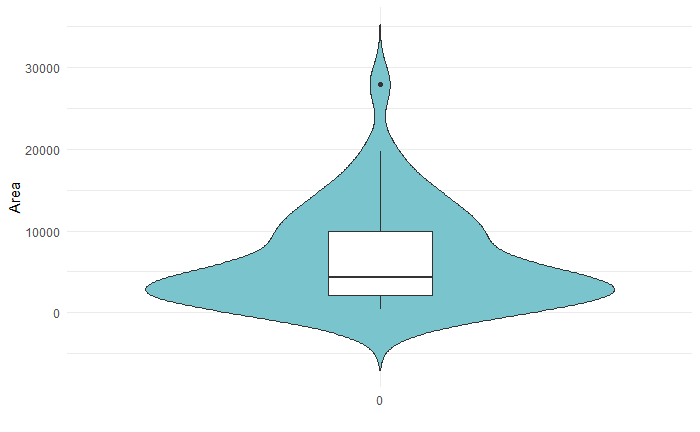
\includegraphics[width=\textwidth]{immagini/vp_area.png}
        \captionsetup{justification=centering}
        \caption{Violinplot della variabile\\ \texttt{Area}}
    \end{minipage}
\end{figure}
La variabile \texttt{Species}, rappresentante il numero di specie di cozze nel fiume, ha una distribuzione asimmetrica a destra come evidenziato dal violinplot \textit{(Figura 1)}. Ha un valore minimo di 2 specie (nel fiume Waccasassa) e un massimo di 33 specie (nel fiume Apalachicola). La mediana è di 10 specie, la media è di 11.25 specie.
La variabile \texttt{Area} segue una distribuzione asimmetrica a destra \textit{(Figura 2)}, con un valore minimo di 349 sq mi \textit{(square mile)} e un massimo di 27900 sq mi. La mediana è di 4315 sq mi, la media è di 6590 sq mi \textit{(Tabella 1)}.

\begin{figure}[H]
    \centering
    \begin{minipage}{0.49\textwidth}
        \centering
        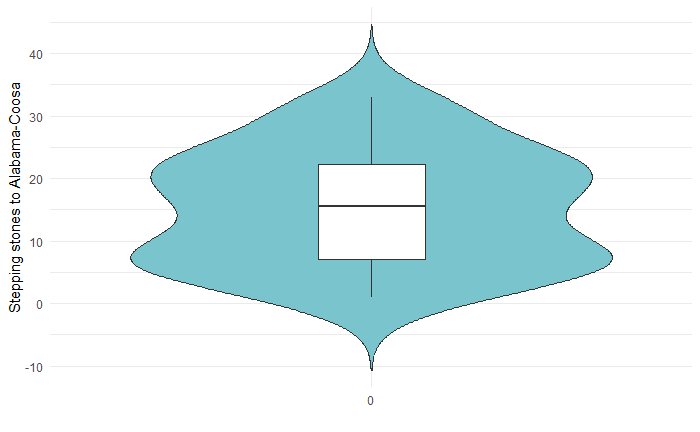
\includegraphics[width=\textwidth]{immagini/vp_ac.png}
        \captionsetup{justification=centering}
        \caption{Violinplot della variabile \texttt{Stepping stones to AC}}
    \end{minipage}
    \hfill
    \begin{minipage}{0.49\textwidth}
        \centering
        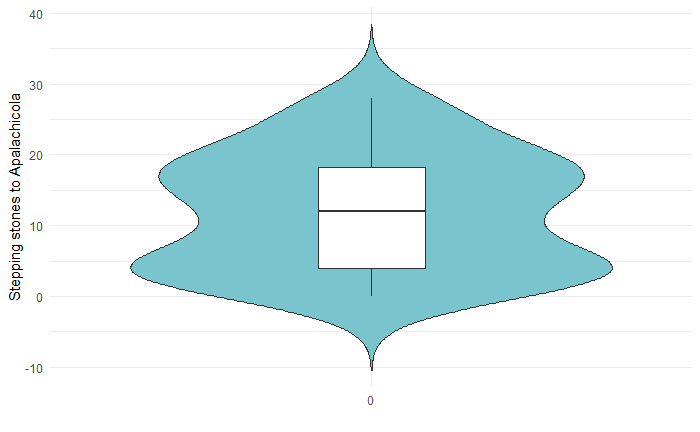
\includegraphics[width=\textwidth]{immagini/vp_ap.png}
        \captionsetup{justification=centering}
        \caption{Violinplot della variabile \texttt{Stepping stones to AP}}
    \end{minipage}
\end{figure}
La distanza dal sistema fluviale di Alabama-Coose (\texttt{Stepping stones to AC}) segue una distribuzione simmetrica \textit{(Figura 3)}, suggerendo che i fiumi sono equamente distribuiti rispetto a questo sistema fluviale. La distanza minima è di 1 e la massima di 33. La idstanza media è di 15.34, e quella mediana di 15.50 "saltelli".
Anche la distanza dal fiume Apalachicola (\texttt{Stepping stones to AP}) segue una distribuzione simmetrica \textit{(Figura 4)}, con una distanza minima di 0 (coincidente con il fiume stesso) e una massima di 28. La distanza media è di 12.02, e quella mediana di 12.00 "saltelli" \textit{(Tabella 1)}.

\begin{figure}[H]
    \centering
    \begin{minipage}{0.49\textwidth}
        \centering
        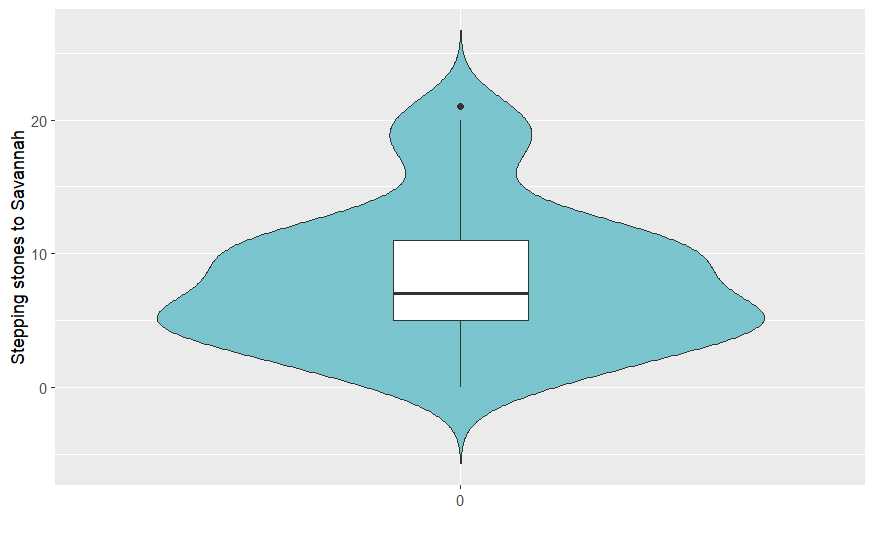
\includegraphics[width=\textwidth]{immagini/vp_sv.png}
        \captionsetup{justification=centering}
        \caption{Violinplot della variabile \texttt{Stepping stones to SV}}
    \end{minipage}
    \hfill
    \begin{minipage}{0.49\textwidth}
        \centering
        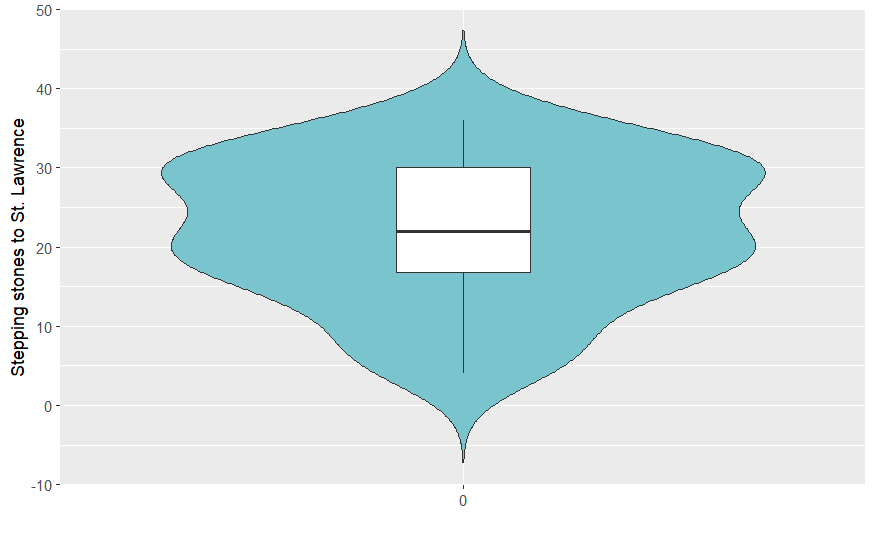
\includegraphics[width=\textwidth]{immagini/vp_sl.png}
        \captionsetup{justification=centering}
        \caption{Violinplot della variabile \texttt{Stepping stones to SL}}
    \end{minipage}
\end{figure}
La distanza dal fiume Savannah (\texttt{Stepping stones to SV}) ha una distribuzione simmetrica anche se presenta una leggera coda lunga a destra \textit{(Figura 5)}, con una distanza minima di 0 (coincidente con il fiume stesso) e una massima di 21. La distanza media è di 8.136, e quella mediana di 7.00. Il valore molto basso della mediana e la presenza di una piccola coda lunga a destra suggeriscono che la maggior parte dei fiumi osservati sono molto vicini al fiume Savannah.
La distanza dal fiume St.\ Lawrence (\texttt{Stepping stones to SL}) ha una distribuzione simmetrica \textit{(Figura 6)}, ma presenta anche una leggera coda lunga a sinistra. La distanza minima di 4 e una massima di 36. La distanza media è di 22.16, e quella mediana di 22.00. Il valore elevato della di media e mediana, in aggiunta alla leggera coda a sinistra, suggerisce che la maggior parte dei fiumi sono distanti al fiume St. Lawrence \textit{(Tabella 1)}.


\begin{figure}[H]
    \centering
    \begin{minipage}{0.49\textwidth}
        \centering
        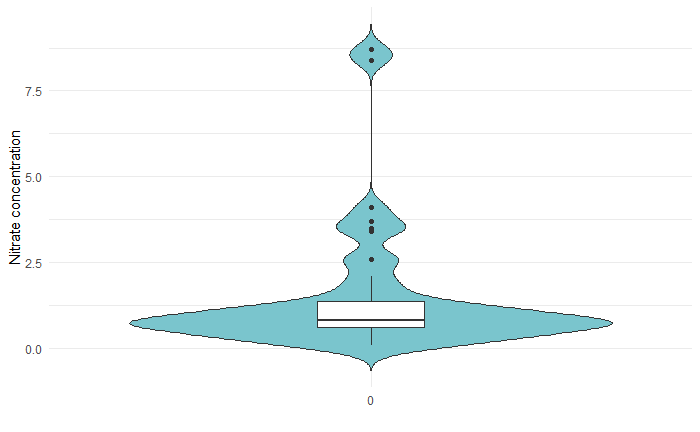
\includegraphics[width=\textwidth]{immagini/vp_nitrate.png}
        \captionsetup{justification=centering}
        \caption{Violinplot della variabile \texttt{Nitrate}}
    \end{minipage}
    \hfill
    \begin{minipage}{0.49\textwidth}
        \centering
        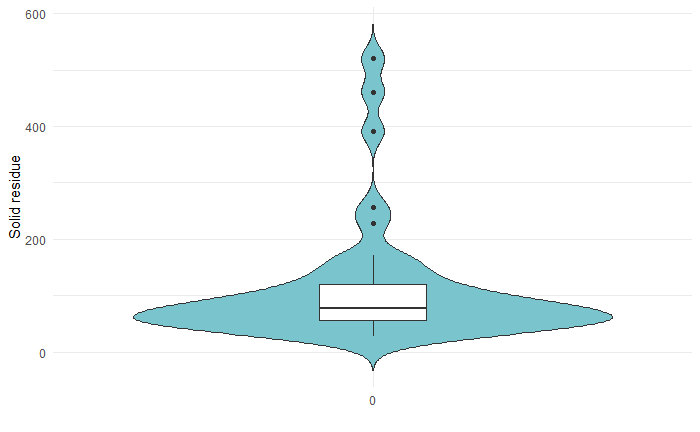
\includegraphics[width=\textwidth]{immagini/vp_sd.png}
        \captionsetup{justification=centering}
        \caption{Violinplot della variabile \texttt{Solid Residue}}
    \end{minipage}
\end{figure}
La variabile \texttt{Nitrate} ha una distribuzione asimmetrica a destra \textit{(Figura 7)}, con un valore minimo di 0.100 ppm \textit{(parts per million)} e un massimo di 8.700 ppm. La mediana è di 0.800 ppm, la media è di 1.495 ppm.
la variabile \texttt{Solid Residue} ha anche essa una distribuzione asimmetrica a destra \textit{(Figura 8)}, con un valore minimo di 29.0 ppm e un massimo di 520.0 ppm. La mediana è di 78.0 ppm, la media è di 112.4 ppm \textit{(Tabella 1)}.


\begin{figure}[H]
    \centering
    \begin{minipage}{0.49\textwidth}
        \centering
        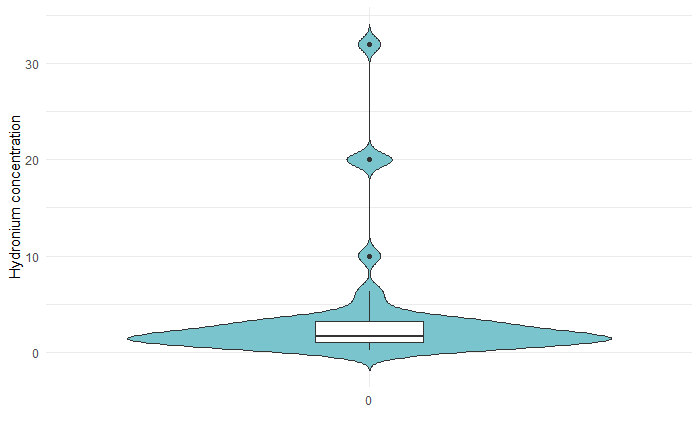
\includegraphics[width=\textwidth]{immagini/vp_hy.png}
        \captionsetup{justification=centering}
        \caption{Violinplot della variabile \texttt{Hydronium}}
    \end{minipage}
    \hfill
    \begin{minipage}{0.49\textwidth}
        \centering
        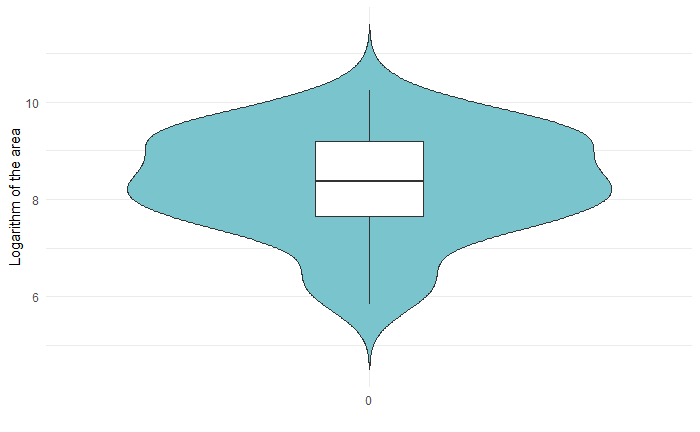
\includegraphics[width=\textwidth]{immagini/vp_ln.png}
        \captionsetup{justification=centering}
        \caption{Violinplot della variabile \texttt{ln(Area)}}
    \end{minipage}
\end{figure}
La variabile \texttt{Hydronium} ha una distribuzione asimmetrica a destra \textit{(Figura 9)}, con un valore minimo di 0.200 e un massimo di 32.00. La mediana è di 1.600, la media è di 3.631.
La variabile \texttt{ln(Area)} segue una distribuzione simmetrica \textit{(Figura 10)}, con un valore minimo di 5.855 e un massimo di 10.24. La mediana è di 8.370, la media è di 8.331 \textit{(Tabella 1)}.


%Seconda parte: analisi bivariate
%Titolo
\newpage
\begin{flushleft}
    
    \textbf{\Large 1.2 \: Analisi Bivariate}
    \vskip 10pt
\end{flushleft}
\vskip 10pt

%Introduzione analisi bivariate
Si valuta la relazione tra le varie variabili. Delle 36 bivariate totali, 16 bivariate sono risultate significative \textit{(Tabella 2)}.\\

\begin{table}[H]
    \centering
    \renewcommand{\arraystretch}{1.4} % Increases the row height
    % \begin{tabularx}{\textwidth}{p{69pt}l p{30pt}c p{45pt}c p{35pt}c p{40pt}c p{30pt}c p{27pt}r}
    \begin{tabular}{lcccccccc}
        \toprule
        & \texttt{ln(A)} & \texttt{H\textsuperscript{+}} & \texttt{SR} & \texttt{NO\textsubscript{3}} & \texttt{SL} & \texttt{SV} & \texttt{AP} & \texttt{AC}\\
        % & & & \texttt{Residue}& & \texttt{stones to SL} & \texttt{stones to SV} & \texttt{stones to AP} & \texttt{stones to AC} &\\
        \midrule  
            % \texttt{Species} & 1 & 0 & 0 & 0 & 0 & 0 & 0 & 0\\
            % \texttt{Stepping stones to AC} & 0 & 1 & 0 & 1 & 1 & 1 & 1 \\
            % \texttt{Stepping stones to AP} & 0 & 1 & 0 & 1 & 1 & 1 &  \\
            % \texttt{Stepping stones to SV} & 0 & 0 & 0 & 1 & 1 &  &  \\
            % \texttt{Stepping stones to SL} & 0 & 1 & 0 & 1 &  &  &  \\
            % \texttt{Nitrate} & 0 & 0 & 1 &  &  &  &  \\
            % \texttt{Solid Residue} & 0 & 1 &  &  &  &  &  \\
            % \texttt{Hydronium} & 0 &  &  &  &  &  &  \\
            \texttt{Sp} & 1 & 0 & 0 & 0 & 0 & 0 & 0 & 0\\
            \texttt{AC} & 0 & 1 & 0 & 1 & 1 & 1 & 1 \\
            \texttt{AP} & 0 & 1 & 0 & 1 & 1 & 1 &  \\
            \texttt{SV} & 0 & 0 & 0 & 1 & 1 &  &  \\
            \texttt{SL} & 0 & 1 & 0 & 1 &  &  &  \\
            \texttt{NO\textsubscript{3}} & 0 & 0 & 1 &  &  &  &  \\
            \texttt{SR} & 0 & 1 &  &  &  &  &  \\
            \texttt{H\textsuperscript{+}} & 0 &  &  &  &  &  &  \\
        \bottomrule
    \end{tabular}
    \caption{Tabella che indica la significatività delle bivariate, 1 indica una bivariata significativa, 0 indica una bivariata non significativa, 
    In particolare Sp: \texttt{Species}, AC: \texttt{Stepping stones to AC}, AP: \texttt{Stepping stones to AP}, SV:\ \texttt{Stepping stones to SV}, SL:\ \texttt{Stepping stones to SL}, NO\textsubscript{3}: Nitrate, SR:\ \texttt{Solid Residue}, H\textsuperscript{+}: \texttt{Hydronium}, ln(A): \texttt{ln(Area)}}
    \end{table}

\begin{figure}[H]
    \centering
    \begin{minipage}{0.49\textwidth}
        \centering
        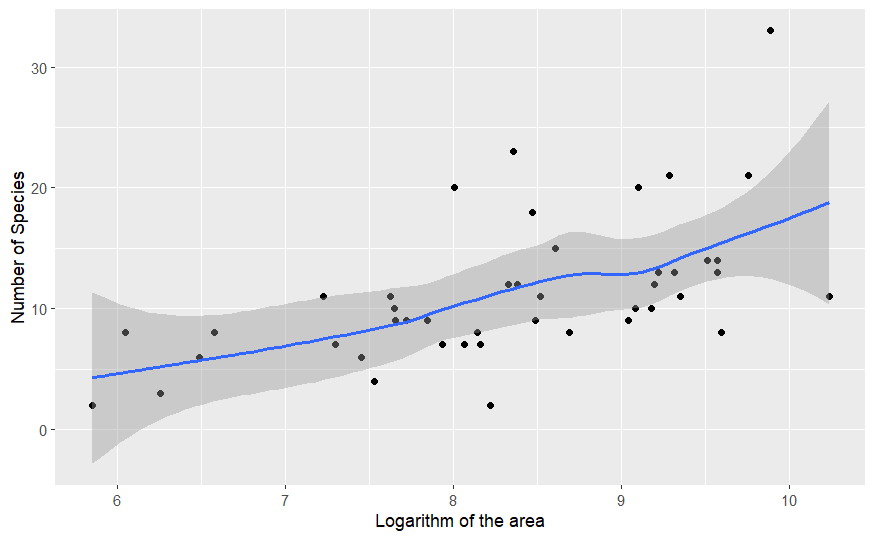
\includegraphics[width=\textwidth]{immagini/sp_ln.png}
        \captionsetup{justification=centering}
        \caption{Diagrammma di dispersione tra \texttt{Species} e \texttt{ln(Area)}, con curva LOESS \textit{(LOcally Estimated Scatterplot Smoothing)} in blu e intervallo di confidenza al 95\% in grigio}
    \end{minipage}
    \hfill
    \begin{minipage}{0.49\textwidth}
        \centering
        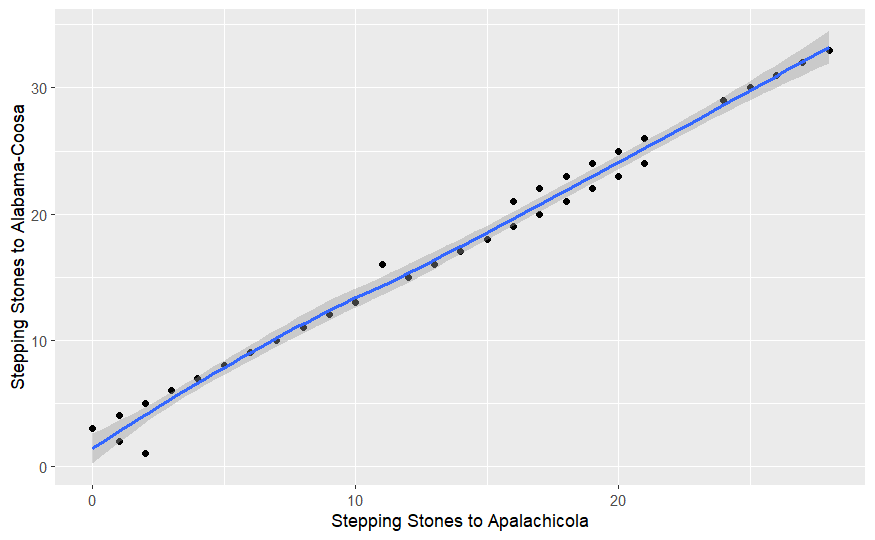
\includegraphics[width=\textwidth]{immagini/ac_ap.png}
        \captionsetup{justification=centering}
        \caption{Diagramma di dispersione tra \texttt{Stepping stones to AC} e \texttt{Stepping stones to AP}, con curva LOESS in blu e intervallo di confidenza \\al 95\% in grigio}
    \end{minipage}
\end{figure}
Dal diagramma di dispersione tra il numero di specie di cozze e il logaritmo dell'area \textit{(Figura 11)} si nota una relazione positiva tra le due variabili.  
La correlazione di Spearman è 0.64, indicando una relazione positiva tra le due variabili; dunque all'aumentare del logaritmo dell'area del fiume aumenta anche il numero di specie di cozze presenti.
Il test per verificare se la correlazione è significativa (S=5089.2, p-value=0.00001) porta a rifiutare l'ipotesi che la correlazione non sia significativa che conferma la presenza di una relazione positiva tra le due variabili.

Dal diagramma di dispersione tra la distanza dei vari fiumi osservati dal sistema fluviale Alabama-Coose e dal fiume Apalachicola \textit{(Figura 12)} si nota una relazione positiva, quasi lineare, tra le due variabili.  
La correlazione di Spearman è 0.99, indicando una forte relazione positiva tra le due variabili; dunque all'aumentare della distanza di un fiume dal sistema fluviale Alabama-Coose aumenta anche la distanza dal fiume Apalachicola. 
Questa relazione è dovuta al fatto che i due fiumi sono molto vicini tra loro, scorrono in parallelo, e sfociano entrambi nel Golfo del Messico, e quindi la distanza da uno implica la distanza dall'altro.
Il test per verificare se la correlazione è significativa (S=89.42, p-value=0.00001) porta a rifiutare l'ipotesi che la correlazione non sia significativa.


\begin{figure}[H]
    \centering
    \begin{minipage}{0.49\textwidth}
        \centering
        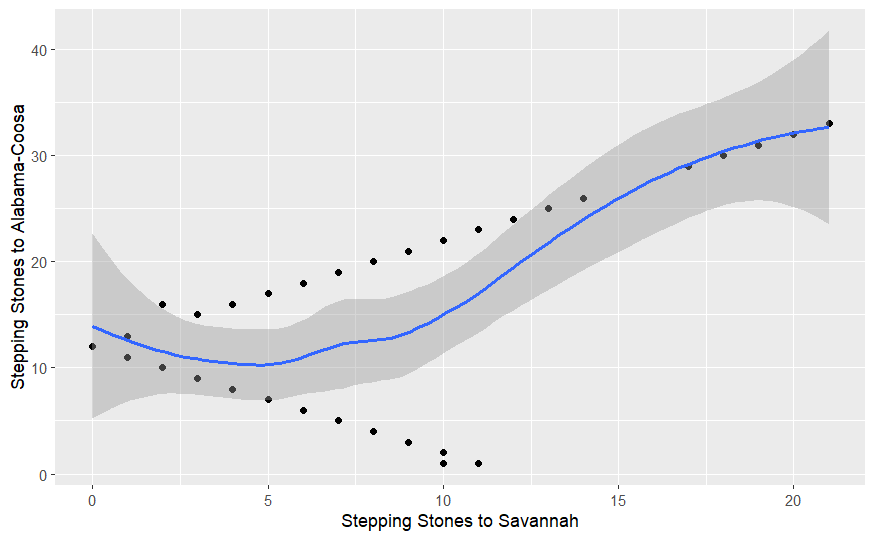
\includegraphics[width=\textwidth]{immagini/ac_sv.png}
        \captionsetup{justification=centering}
        \caption{Diagrammma di dispersione tra \texttt{Stepping stones to AC} e \texttt{Stepping stones to SV}, con curva LOESS in blu e intervallo di confidenza al 95\% in grigio}
    \end{minipage}
    \hfill
    \begin{minipage}{0.49\textwidth}
        \centering
        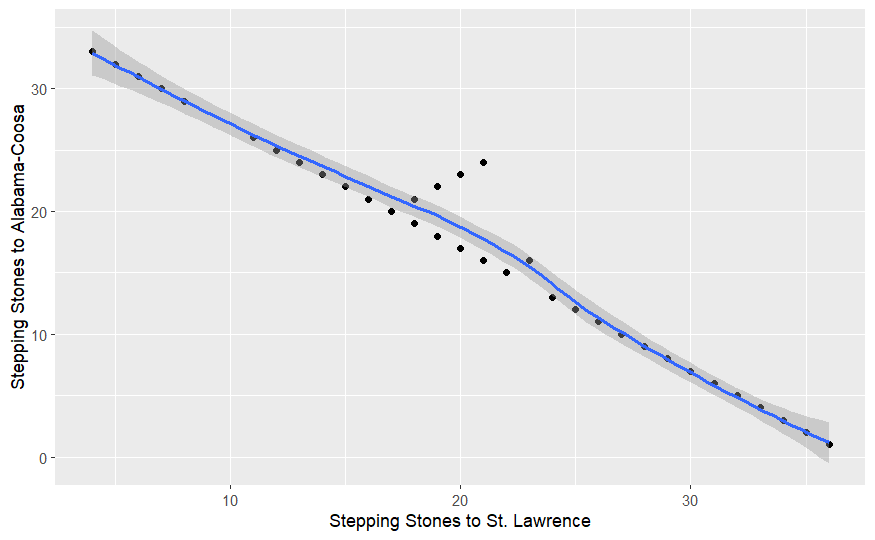
\includegraphics[width=\textwidth]{immagini/ac_sl.png}
        \captionsetup{justification=centering}
        \caption{Diagramma di dispersione tra \texttt{Stepping stones to AC} e \texttt{Stepping stones to SL}, con curva LOESS in blu e intervallo di confidenza al 95\% in grigio}
    \end{minipage}
\end{figure}

Dal diagramma di dispersione tra la distanza dei vari fiumi osservati dal sistema fluviale Alabama-Coose e dal fiume Savannah \textit{(Figura 13)} si nota una relazione tendenzialmente positiva, ma molto curvilinea tra le due variabili. 
In particolare si nota come nella prima del grafico i punti divergono tra di loro. Questo è dovuto al fatto che il fiume Savannah e il sistema fluviale Alabama-Coose scorrono perpendicolarmente tra di loro, quasi a formare un angolo retto. Quindi una porzione di fiumi (quelli situati a Sud), mentre si allontananano dal fiume Savannah si avvicinano al sistema fluviale Alabama-Coose. Al contrario, i fiumi situati a Nord si allontananano parallamente ad entrambi i fiumi che spiega la crescita positiva nella seconda parte del grafico.
La correlazione di Spearman è 0.54, indicando una modesta relazione positiva tra le due variabili. La correlazione è positiva; dunque all'aumentare della distanza di un fiume dal sistema fluviale Alabama-Coose aumenta anche la distanza dal fiume Savannah. 
Il test per verificare se la correlazione è significativa (S=6483.6, p-value=0.0001) porta a rifiutare l'ipotesi che la correlazione non sia significativa.

Dal diagramma di dispersione tra la distanza dei vari fiumi osservati dal sistema fluviale Alabama-Coose e dal fiume Saint Lawrence \textit{(Figura 14)} si nota una relazione negativa, abbastanza lineare, tra le due variabili.  
La correlazione di Spearman è -0.97, indicando una forte relazione negativa tra le due variabili; dunque all'aumentare della distanza di un fiume dal sistema fluviale Alabama-Coose diminuisce la distanza dal fiume St. Lawrence. 
Questo è dovuto dalla posizione dei due fiumi. Essi, infatti, si trovano alle due estremità della regione osservata, con il fiume St. Lawrence situato più a Nord-Est e il sistema fluviale Alabama-Coose situato invece a Sud-Ovest. Quindi allontanandosi dal sistema fluviale Alabama-Coose ci si avvicina al fiume St. Lawrence, e viceversa.
Il test per verificare se la correlazione è significativa (S=28075, p-value=0.000001) porta a rifiutare l'ipotesi che la correlazione non sia significativa.

\begin{figure}[H]
    \centering
    \begin{minipage}{0.49\textwidth}
        \centering
        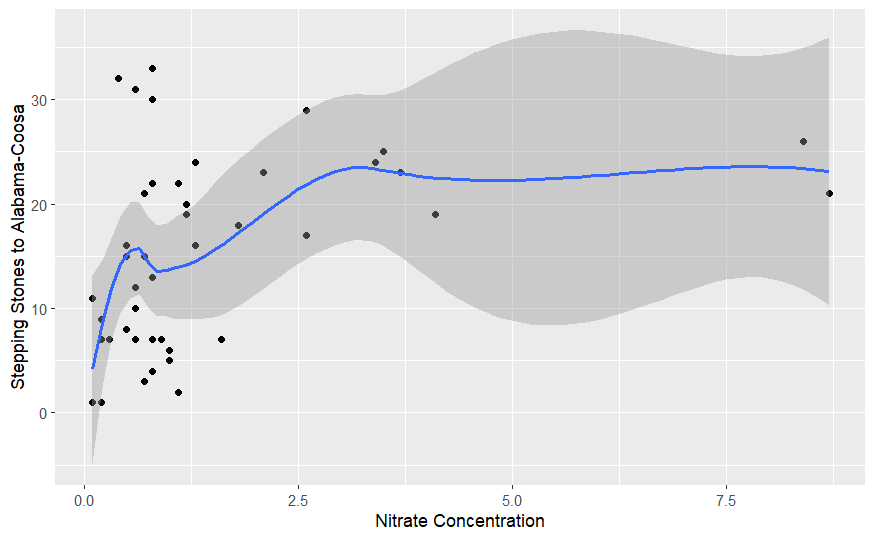
\includegraphics[width=\textwidth]{immagini/ac_nitrate.png}
        \captionsetup{justification=centering}
        \caption{Diagrammma di dispersione tra \texttt{Stepping stones to AC} e \texttt{Nitrate}, con curva LOESS in blu e intervallo di confidenza al 95\% in grigio}
    \end{minipage}
    \hfill
    \begin{minipage}{0.49\textwidth}
        \centering
        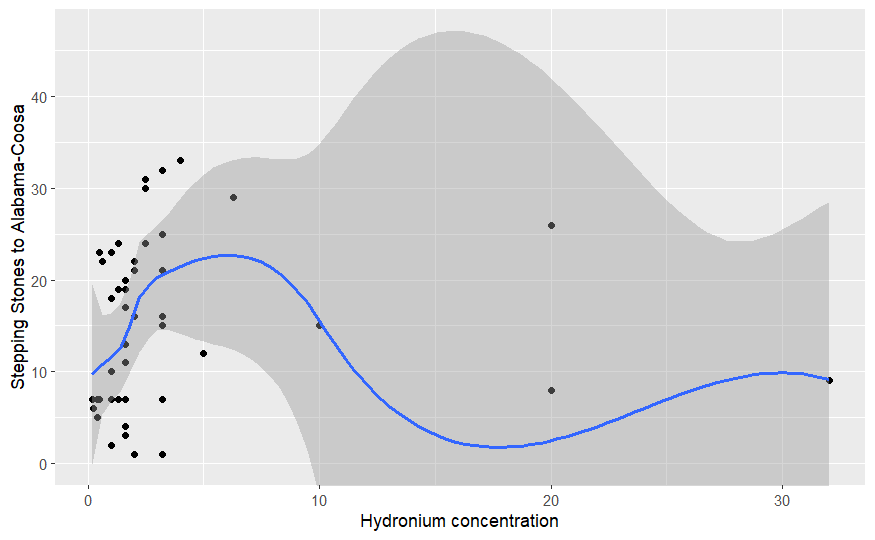
\includegraphics[width=\textwidth]{immagini/ac_hy.png}
        \captionsetup{justification=centering}
        \caption{Diagramma di dispersione tra \texttt{Stepping stones to AC} e \texttt{Hydronium}, con curva LOESS in blu e intervallo di confidenza al 95\% in grigio}
    \end{minipage}
\end{figure}

Dal diagramma di dispersione tra la distanza dei vari fiumi osservati dal sistema fluviale Alabama-Coose e la concentrazione di nitrato nelle acque dei fiumi osservati \textit{(Figura 15)} si osserva una relazione molto curvilinea.
In particolare si nota come i fiumi più vicini al sistema fluviale Alabama-Coose presentano una minore concentrazione di nitrato. La concentrazione di nitrato aumenta all'aumentare della distanza dal sistema fluviale Alabama-Coose, ma solo fino ad un certo punto. Infatti, dopo una certa distanza, la concentrazione di nitrato inizia a diminuire.
La correlazione di Spearman è 0.42, indicando una lieve relazione positiva tra le due variabili. 
Il test per verificare se la correlazione è significativa (S=8173.9, p-value=0.004) porta a rifiutare l'ipotesi che la correlazione non sia significativa.

Dal diagramma di dispersione tra la distanza dei vari fiumi osservati dal sistema fluviale Alabama-Coose e la variabile \texttt{Hydronium} \textit{(Figura 16)} si nota come la maggior parte dei fiumi presenti valori bassi di concentrazione di idronio. Fanno eccezione 5 fiumi che invece presentano valori molto alti di concentrazione di idronio. 
La correlazione di Spearman è 0.33, indicando una lieve relazione positiva tra le due variabili. 
Il test per verificare se la correlazione è significativa (S=9506.5, p-value=0.029) porta a rifiutare l'ipotesi che la correlazione non sia significativa al 5\%, ma non all'1\%.

\begin{figure}[H]
    \centering
    \begin{minipage}{0.49\textwidth}
        \centering
        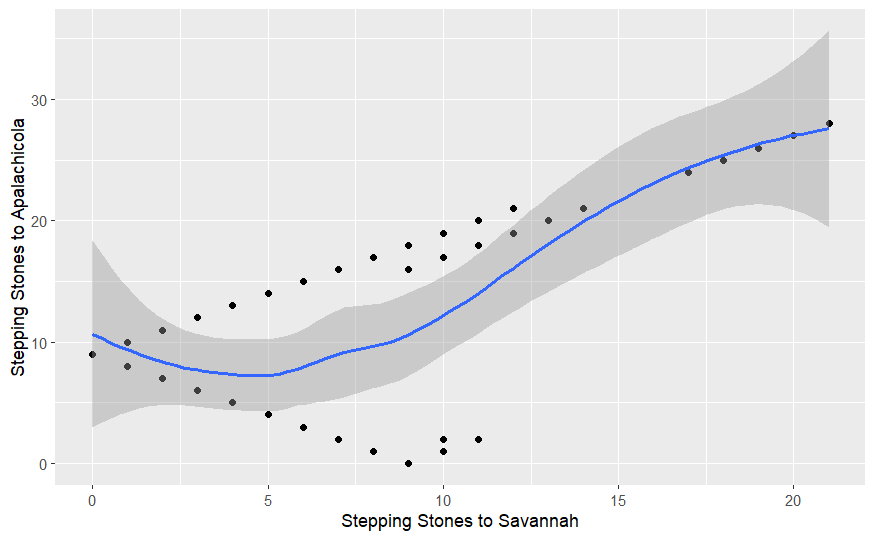
\includegraphics[width=\textwidth]{immagini/ap_sv.png}
        \captionsetup{justification=centering}
        \caption{Diagrammma di dispersione tra \texttt{Stepping stones to AP} e \texttt{Stepping stones to SV}, con curva LOESS in blu e intervallo di confidenza al 95\% in grigio}
    \end{minipage}
    \hfill
    \begin{minipage}{0.49\textwidth}
        \centering
        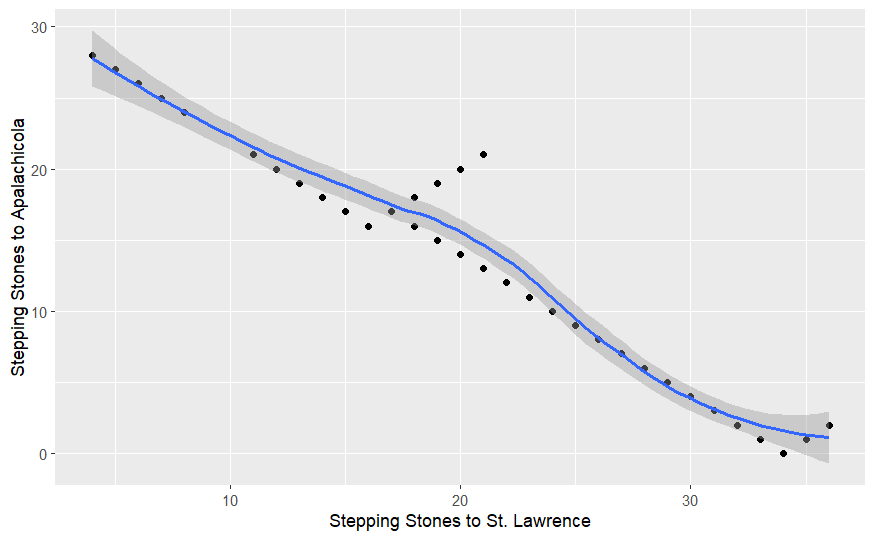
\includegraphics[width=\textwidth]{immagini/ap_sl.png}
        \captionsetup{justification=centering}
        \caption{Diagramma di dispersione tra \texttt{Stepping stones to AP} e \texttt{Stepping stones to SL}, con curva LOESS in blu e intervallo di confidenza al 95\% in grigio}
    \end{minipage}
\end{figure}

Dal diagramma di dispersione tra la distanza dei vari fiumi osservati dal fiume Apalachicola e dal fiume Savannah \textit{(Figura 17)} si nota una relazione tendenzialmente positiva, ma molto curvilinea tra le due variabili. 
Il grafico mostra una situazione simile a quella osservata tra la distanza dei fiumi dal sistema fluviale Alabama-Coose e dal fiume Savannah in \textit{Figura 13}. Anche in questo caso, infatti, si osserva nella prima parte un divergere delle distanze e successivamente un crescere lineare delle stesse. 
Ciò è dovuto alla posizione del fiume Apalachicola che è molto vicino al sistema fluviale Alabama-Coose e quindi questo causa un comportamento simile.
La correlazione di Spearman è 0.55, indicando una modesta relazione positiva tra le due variabili.  
Il test per verificare se la correlazione è significativa (S=6436.4, p-value=0.0001) porta a rifiutare l'ipotesi che la correlazione non sia significativa.

Dal diagramma di dispersione tra la distanza dei vari fiumi osservati dal fiume Apalachicola e dal fiume Saint Lawrence \textit{(Figura 18)} si evince una situazione analoga a quella discussa precedentemente.
Si nota una relazione negativa, abbastanza lineare, tra le due variabili molto simile a quella in \textit{Figura 14}
La correlazione di Spearman è -0.97, indicando una forte relazione negativa tra le due variabili; dunque all'aumentare della distanza di un fiume dal sistema fluviale Apalachicola diminuisce la distanza dal fiume St. Lawrence. 
Il test per verificare se la correlazione è significativa (S=27892, p-value=0.000001) porta a rifiutare l'ipotesi che la correlazione non sia significativa.

\begin{figure}[H]
    \centering
    \begin{minipage}{0.49\textwidth}
        \centering
        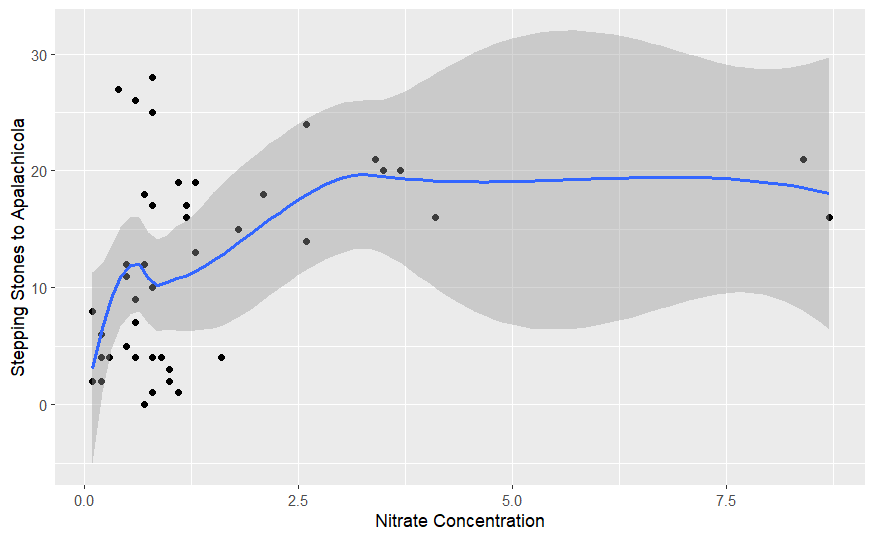
\includegraphics[width=\textwidth]{immagini/ap_nitrate.png}
        \captionsetup{justification=centering}
        \caption{Diagrammma di dispersione tra \texttt{Stepping stones to AP} e \texttt{Nitrate}, con curva LOESS in blu e intervallo di confidenza al 95\% in grigio}
    \end{minipage}
    \hfill
    \begin{minipage}{0.49\textwidth}
        \centering
        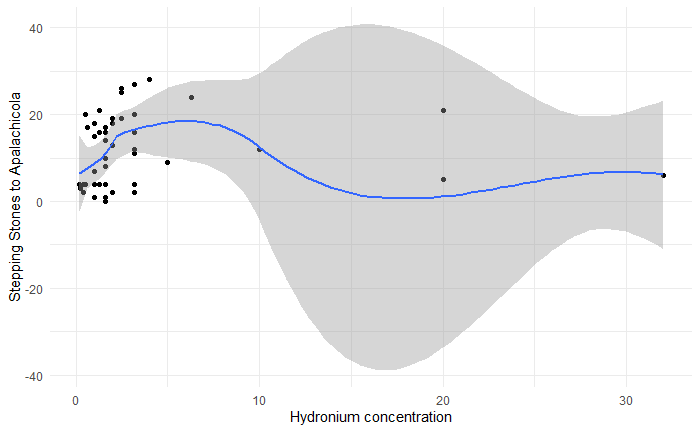
\includegraphics[width=\textwidth]{immagini/ap_hy.png}
        \captionsetup{justification=centering}
        \caption{Diagramma di dispersione tra \texttt{Stepping stones to AP} e \texttt{Hydronium}, con curva LOESS in blu e intervallo di confidenza al 95\% in grigio}
    \end{minipage}
\end{figure}

Dal diagramma di dispersione tra la distanza dei vari fiumi osservati dal fiume Apalachicola e la concentrazione di nitrato nelle acque dei fiumi osservati \textit{(Figura 19)} si nota come i fiumi più vicini al fiume Apalachicola presentano una bassa concentrazione di nitrato, seguita da un aumento di essa mentre ci si allontana dal fiume e infine una diminuzione della concentrazione di nitrato.
La correlazione di Spearman è 0.40, indicando una lieve relazione positiva tra le due variabili. 
Il test per verificare se la correlazione è significativa (S=8454.7, p-value=0.006) porta a rifiutare l'ipotesi che la correlazione non sia significativa.

Dal diagramma di dispersione tra la distanza dei vari fiumi osservati dal fiume Apalachicola e la concentrazione di idronio \textit{(Figura 20)} si nota come la maggior parte dei fiumi sia schiacciata nella prima parte del grafico, con valori bassi di concentrazione di idronio. Solo 5 fiumi, presentano valori molto alti di concentrazione di idronio.
La correlazione di Spearman è 0.33, indicando una lieve relazione positiva tra le due variabili. 
Il test per verificare se la correlazione è significativa (S=9438.8, p-value=0.026) porta a rifiutare l'ipotesi che la correlazione non sia significativa al 5\%.

\begin{figure}[H]
    \centering
    \begin{minipage}{0.49\textwidth}
        \centering
        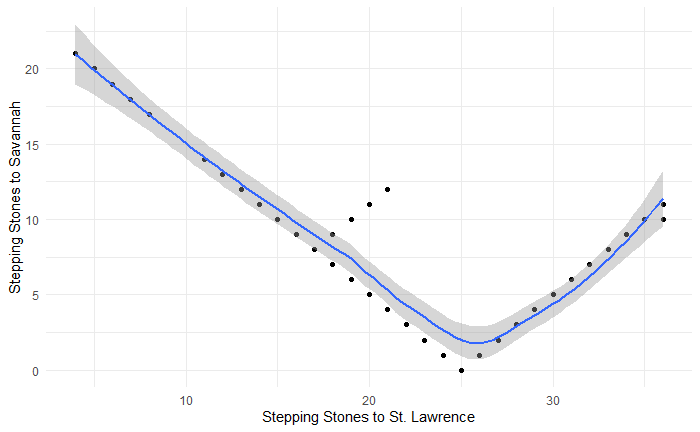
\includegraphics[width=\textwidth]{immagini/sv_sl.png}
        \captionsetup{justification=centering}
        \caption{Diagrammma di dispersione tra \texttt{Stepping stones to SV} e \texttt{Stepping stones to SL}, con curva LOESS in blu e intervallo di confidenza al 95\% in grigio}
    \end{minipage}
    \hfill
    \begin{minipage}{0.49\textwidth}
        \centering
        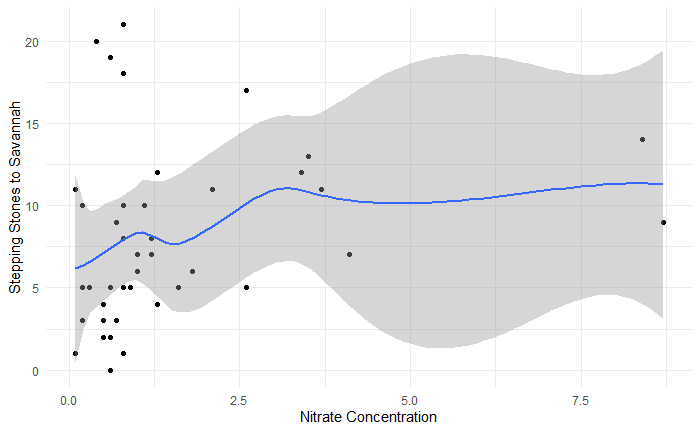
\includegraphics[width=\textwidth]{immagini/sv_nitrate.png}
        \captionsetup{justification=centering}
        \caption{Diagramma di dispersione tra \texttt{Stepping stones to SV} e \texttt{Nitrate}, con curva LOESS in blu e intervallo di confidenza al 95\% in grigio}
    \end{minipage}
\end{figure}

Dal diagramma di dispersione tra la distanza dei vari fiumi osservati dal fiume Savannah e dal fiume St. Lawrence \textit{(Figura 21)} si nota una relazione inizialmente negativa che, una volta raggiunto il fiume Savannah, cambia drasticamente e cresce positivamente. 
Questo andamento è dovuto alla posizione dei due fiumi. Entrambi i fiumi sfociano nell'Atlantico; il fiume St. Lawrence nasce più a Nord, nella regione dei Grandi Laghi e sfocia in Canada, il fiume Savannah invece è situato più a Sud, in Carolina del Sud. La relazione è inizialmente negativa poiché allontanandosi dal fiume St. Lawrence, e procedendo verso Sud, ci si avvicina al fiume Savannah. Una volta raggiunto il fiume Savannah, le distanze tra i due fiumi aumenteranno in parallelo.
La correlazione di Spearman è -0.51, indicando una relazione negativa tra le due variabili.  
Il test per verificare se la correlazione è significativa (S=21406, p-value=0.0004) porta a rifiutare l'ipotesi che la correlazione non sia significativa.

Dal diagramma di dispersione tra la distanza dei vari fiumi osservati dal fiume Savannah e la concentrazione di nitrato nelle acque dei fiumi osservati \textit{(Figura 22)} si nota un andamento simile a quello della \textit{Figura 15} e della \textit{Figura 19}, anche se la curva LOESS appare meno definita. 
Come nella figure precedenti, i fiumi più vicini al fiume Savannah presentano una bassa concentrazione di nitrato, seguita da un aumento di essa mentre ci si allontana dal fiume e infine una diminuzione della concentrazione di nitrato.
La correlazione di Spearman è 0.36, di poco inferiore a quella tra \texttt{Stepping stones to AC} e \texttt{Nitrate} \texttt{Stepping stones to AP} e \texttt{Nitrate} rispettivamente di 0.42 e 0.40. La relazione è lieve ed è positiva. 
Il test per verificare se la correlazione è significativa (S=9025.2, p-value=0.015) porta a rifiutare l'ipotesi che la correlazione non sia significativa.

\begin{figure}[H]
    \centering
    \begin{minipage}{0.49\textwidth}
        \centering
        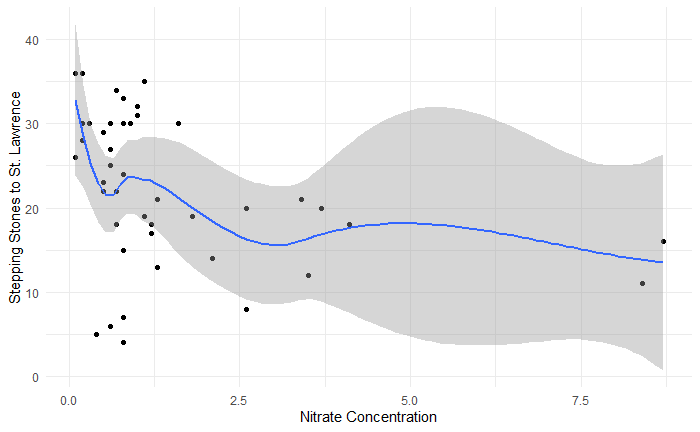
\includegraphics[width=\textwidth]{immagini/sl_nitrate.png}
        \captionsetup{justification=centering}
        \caption{Diagrammma di dispersione tra \texttt{Stepping stones to SL} e \texttt{Nitrate}, con curva LOESS in blu e intervallo di confidenza al 95\% in grigio}
    \end{minipage}
    \hfill
    \begin{minipage}{0.49\textwidth}
        \centering
        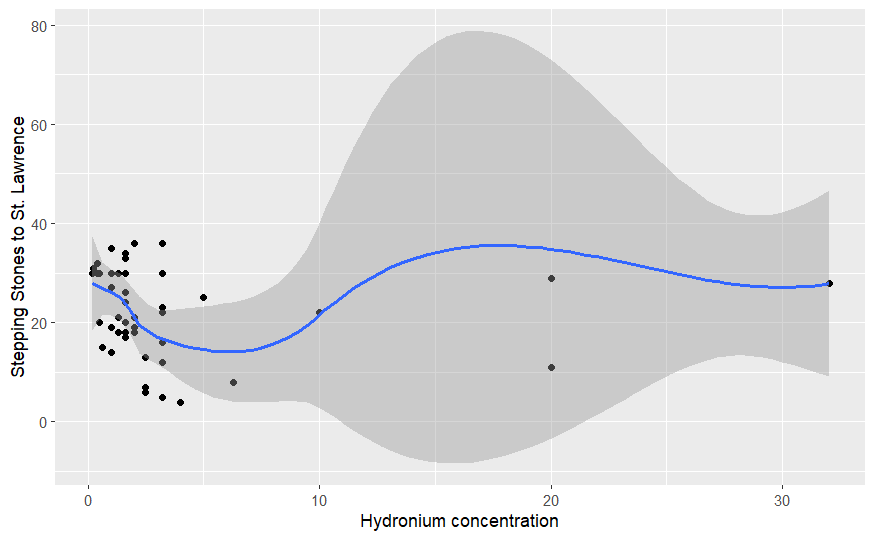
\includegraphics[width=\textwidth]{immagini/sl_hy.png}
        \captionsetup{justification=centering}
        \caption{Diagramma di dispersione tra \texttt{Stepping stones to SL} e \texttt{Hydronium}, con curva LOESS in blu e intervallo di confidenza al 95\% in grigio}
    \end{minipage}
\end{figure}

IL diagramma di dispersione tra la distanza dei vari fiumi osservati dal fiume St. Lawrence e la concentrazione di nitrato nelle acque dei fiumi osservati \textit{(Figura 23)} mostra una situazione capovolta rispetto a quella osservata nelle \textit{Figura 15}, \textit{Figura 19}, \textit{Figura 22}.
Il capovolgimento è dovuto al fatto che il fiume St. Lawrence è situato più a Nord-Est rispetto agli altri fiumi osservati. Quindi i valori che si trovavano distanti dagli altri fiumi, ora sono vicini al fiume St. Lawrence e viceversa. 
La correlazione di Spearman è -0.41. La correlazione è negativa, ma al netto del segno, è in linea con le correlazioni tra gli altri fiumi e la concentrazione di nitrato.  
Il test per verificare se la correlazione è significativa (S=20062, p-value=0.005) porta a rifiutare l'ipotesi che la correlazione non sia significativa.

Dal diagramma di dispersione tra la distanza dei vari fiumi osservati dal fiume St. Lawrence e la concentrazione di idronio \textit{(Figura 24)} si nota come la situazione, analogamente alla \textit{Figura 23}, sia capovolta rispetto a quella osservata nelle \textit{Figura 16} e \textit{Figura 20}.
La correlazione di Spearman è -0.35, indicando una lieve relazione negativa tra le due variabili. 
Il test per verificare se la correlazione è significativa (S=19135, p-value=0.02) porta a rifiutare l'ipotesi che la correlazione non sia significativa al 5\%.

\begin{figure}[H]
    \centering
    \begin{minipage}{0.49\textwidth}
        \centering
        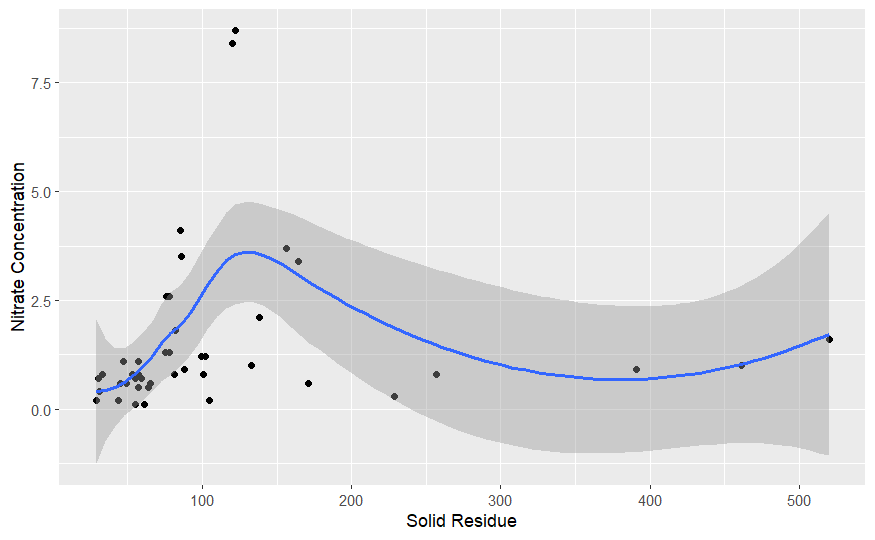
\includegraphics[width=\textwidth]{immagini/sr_nitrate.png}
        \captionsetup{justification=centering}
        \caption{Diagrammma di dispersione tra \texttt{Nitrate} e \texttt{Solid Residue}, con curva LOESS in blu e intervallo di confidenza al 95\% in grigio}
    \end{minipage}
    \hfill
    \begin{minipage}{0.49\textwidth}
        \centering
        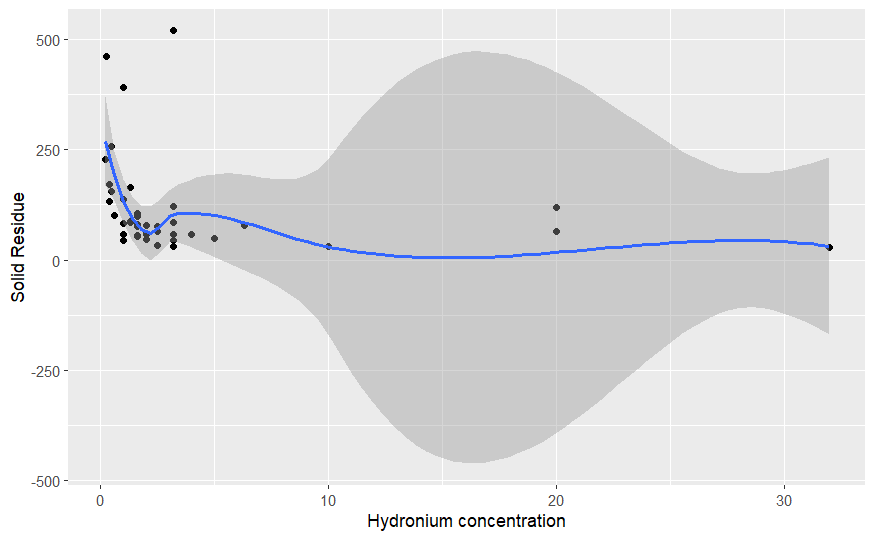
\includegraphics[width=\textwidth]{immagini/sr_hy.png}
        \captionsetup{justification=centering}
        \caption{Diagramma di dispersione tra \texttt{Solid Residue} e \texttt{Hydronium}, con curva LOESS in blu e intervallo di confidenza al 95\% in grigio}
    \end{minipage}
\end{figure}

Dal diagramma di dispersione tra la concentrazione di nitrato e la concentrazione di residuo solido nelle acque dei fiumi osservati \textit{(Figura 25)} si osserva un iniziale aumento della concentrazione di idronio all'aumentare della concentrazione di residuo solido. Tuttavia, dopo un certo punto (intorno al valore 15 per il residuo solido), la concentrazione di nitrato inizia a diminuire.
La correlazione di Spearman è 0.50, indicando una modesta relazione positiva tra le due variabili. 
Il test per verificare se la correlazione è significativa (S=7386.3, p-value=0.001) porta a rifiutare l'ipotesi che la correlazione non sia significativa al 5\%, ma non all'1\%.

Dal diagramma di dispersione tra la concentrazione di residuo solido e la variabile \texttt{Hydronium} \textit{(Figura 26)} si nota una relazione molto ondulatoria tra le due variabili.
La correlazione è nel complesso (tranne in una piccola parte del grafico tra i valori 2 e 3) negativa.
La correlazione di Spearman è -0.55, confermando la presenza di una modesta relazione negativa tra le due variabili. Dunque, all'aumentare della concentrazione di residuo solido diminuisce la concentrazione di idronio.
Questo andamento ha molto senso in quanto il residuo solido è composto da sostanze base, al contrario l'idronio è un acido, essendo ance legato al calcolo del pH. Quindi all'aumentare della concentrazione di parte base, la concentrazione di acido diminuisce.
Il test per verificare se la correlazione è significativa (S=21968, p-value=0.0001) porta a rifiutare l'ipotesi che la correlazione non sia significativa al 5\%, ma non all'1\%.



\end{document}
%         \centering
%         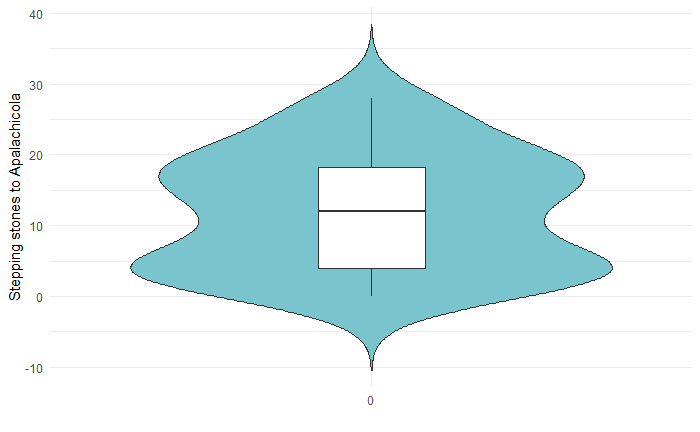
\includegraphics[width=\textwidth]{immagini/vp_ap.png}
%         \captionsetup{justification=centering}
%         \caption{Violinplot della variabile \texttt{stepping stones to AP}}
%     \end{minipage}
%     \hfill
%     \begin{minipage}{0.30\textwidth}
%         \centering
%         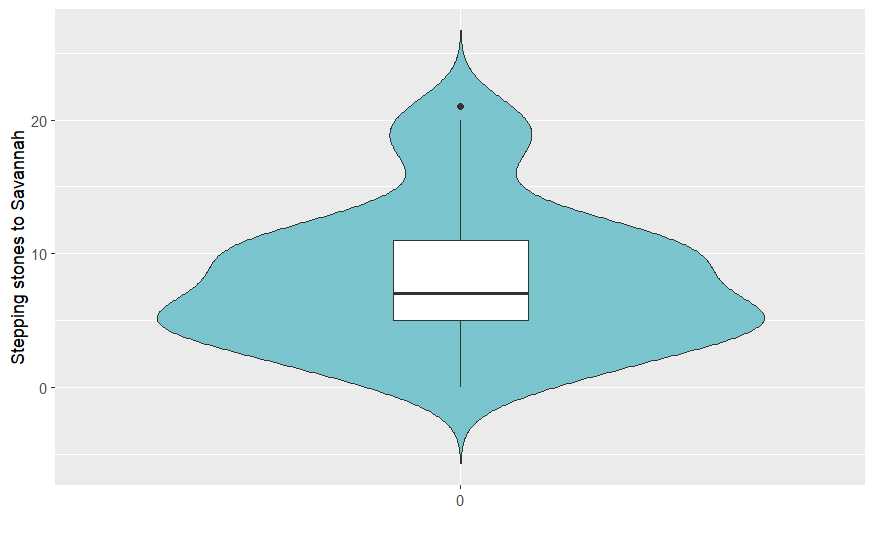
\includegraphics[width=\textwidth]{immagini/vp_sv.png}
%         \captionsetup{justification=centering}
%         \caption{Violinplot della variabile \texttt{stepping stones to SV}}
%     \end{minipage}
%     \hfill
%     \begin{minipage}{0.30\textwidth}
%         \centering
%         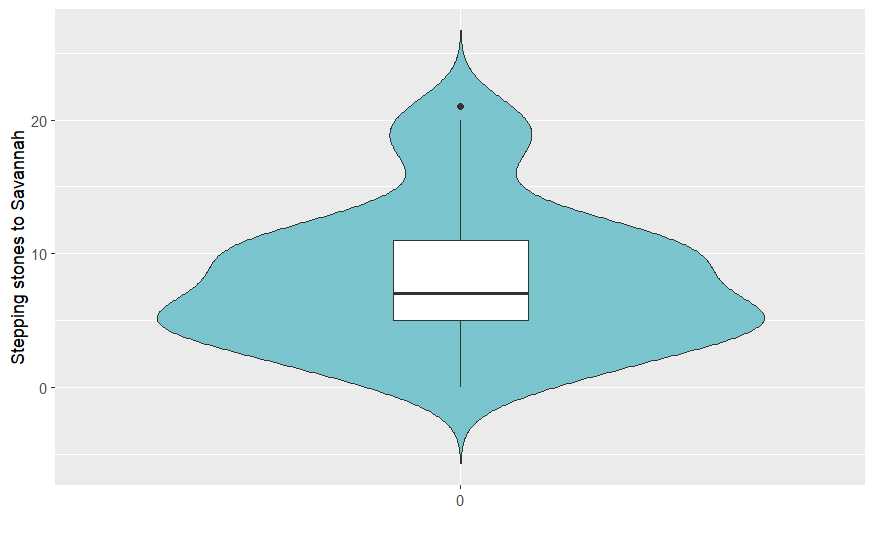
\includegraphics[width=\textwidth]{immagini/vp_sv.png}
%         \captionsetup{justification=centering}
%         \caption{Violinplot della variabile \texttt{stepping stones to SV}}
%     \end{minipage}
% \end{figure}